\section{Price-dividend ratio and return predictability}
 Given that the valuation ratio is linear in the consumption share, the price-dividend ratio (or wealth-consumption ratio) predicts returns in our model. The left graph of Figure \ref{fig:StockMarketPredictability} shows that the slope coefficient of the predictability regression is negative and the right graph shows that the $R^2$ is increasing with the predictability horizon. Specifically, the slope is strictly decreasing and the $R^2$ is strictly increasing with disagreement. The intuition is straightforward when looking at the right graph of Figure \ref{fig:VolaRiskPremium2f}. It shows that the equity premium is decreasing with the consumption share and, thus, decreasing with the price-dividend ratio except for very low or very high consumption share realizations which do not occur often.  Moreover, the sensitivity of the equity premium to changes in the price-dividend ratio increases with disagreement and vanishes if there is no disagreement because in this case the equity premium is constant.  Interestingly, we expect the predictive relation to change signs in times of very high or low stock market valuations.\footnote{In the Internet Appendix we show that the model is also consistent with the Black's ``Leverage'' effect, i.e., the conditional volatility is negatively correlated with stock market returns.}

\begin{figure}[H]
\centering
\begin{tabular}{cc}
\includegraphics[width=.4\textwidth]{figures/PDregressionSlope2Dis.eps} &
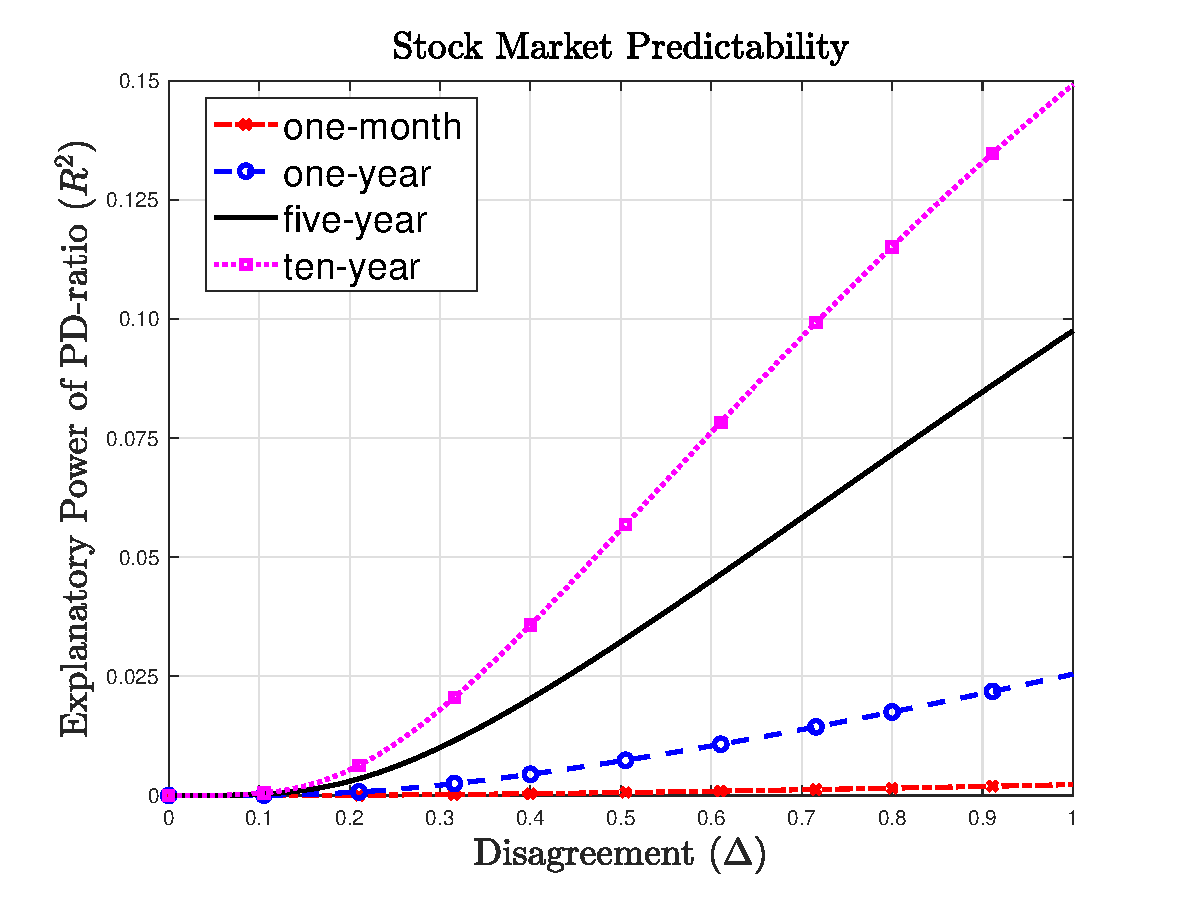
\includegraphics[width=.4\textwidth]{figures/PDregressionRsq2Dis.eps} \\  
\end{tabular}
\caption{\textbf{Stock Market Predictability.}  \footnotesize{The left graph shows the slope and the right graph shows the $R^2$ for the price-divided regressions $Rx_{t,t+\tau} = a + b \phi_t + \epsilon_{t+\tau}$, where $Rx_{t,t+\tau}$ is the excess stock market return from $t$ to $t+\tau$. An increase in the price-dividend ratio lowers expected stock market returns in excess of the risk-free rate. Moreover, the economic significance and explanatory power of this predictive regression is increasing in disagreement.  The slope and $R^2$ are averages based on one million years of monthly observations for each value of disagreement $\Delta$. In this example the parameters are based on the alternative calibration with $\rho^a = 0.001$ and $\rho^b = 0.05$}}  
\label{fig:StockMarketPredictability} 
\end{figure}

\ref{fig:VolaRiskPremium2f} show.
\begin{figure}[H]
\centering
\vspace{0.1in}
\begin{tabular}{cc}
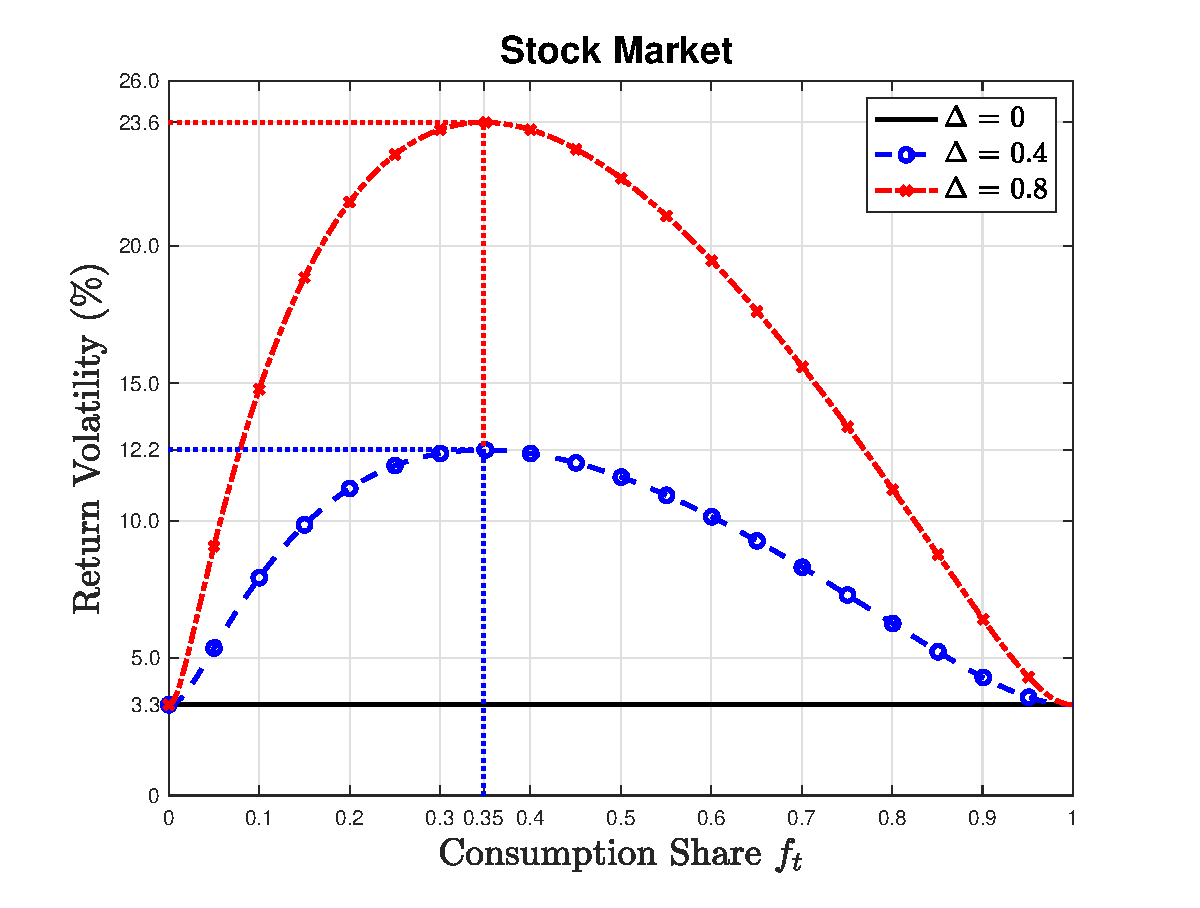
\includegraphics[width=.45\textwidth]{figures/StockMarketVola2f.eps} &
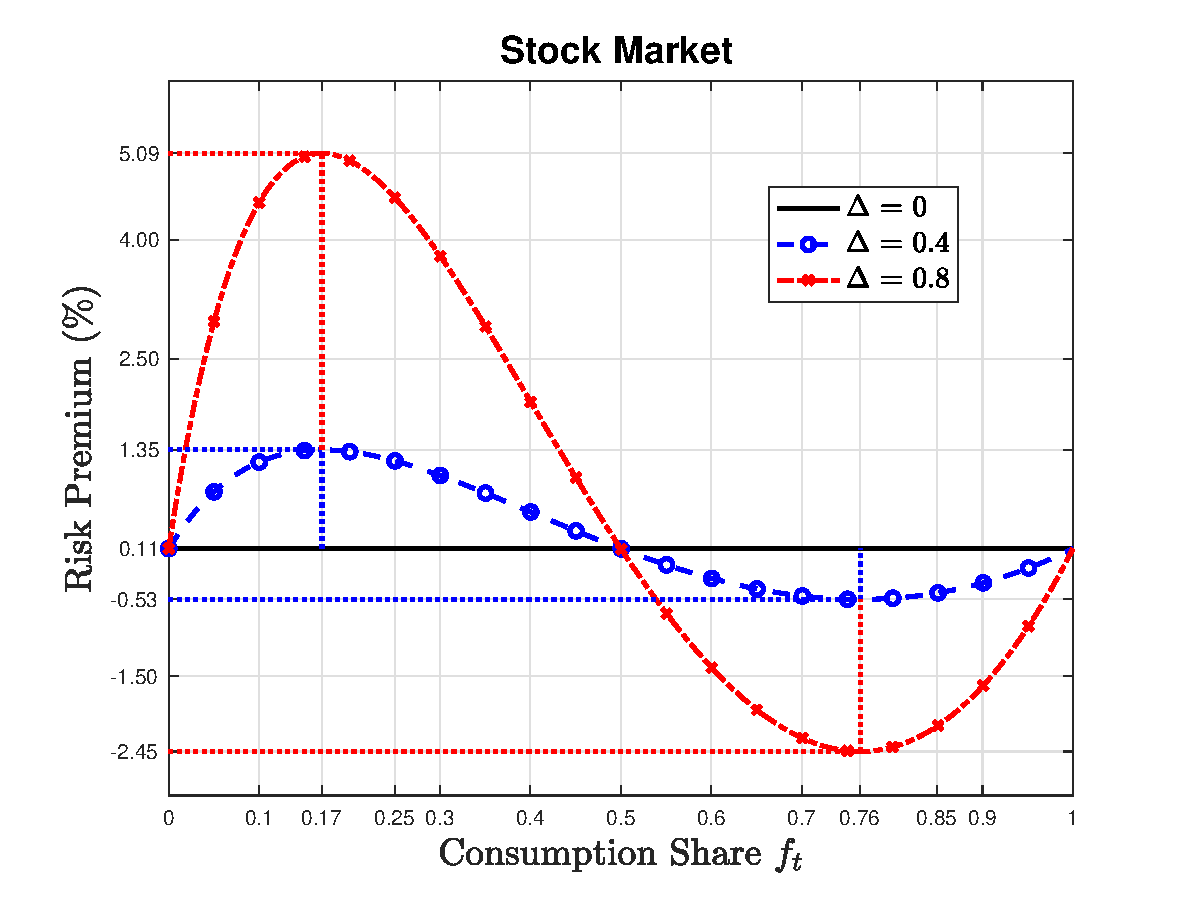
\includegraphics[width=.45\textwidth]{figures/StockMarketRiskPremium2f.eps}
\end{tabular}
\caption{\textbf{Conditional stock market volatility and risk premium.} \footnotesize{The left graph shows stock market volatility and the right graphs shows the equity premium conditional on the consumption share $f_t$ for different disagreement $\Delta$. Disagreement leads to stochastic stock market volatility in excess of output growth volatility and to a stochastic equity premium that is positive if impatient cohorts consume more out of output and negative if patient cohorts consume more out of output. In this example the parameters are based on the alternative calibration with $\rho^a = 0.001$ and $\rho^b = 0.05$}} \label{fig:VolaRiskPremium2f} 
 \end{figure}
